\documentclass[a4paper, 11pt]{article}
\usepackage{geometry}
\usepackage{listings}
\usepackage{url}
\usepackage{here}
\usepackage{subfigure}

\geometry{left=15mm,right=15mm,top=30mm,bottom=20mm}
\usepackage[dvipdfmx]{graphicx}
\renewcommand{\figurename}{Fig}
\newcommand{\figref}[1]{Fig.\hspace{1mm}\ref{#1}}


\begin{document}
\begin{center}
\LARGE{Preferred Networks インターン選考2019\\ コーディング課題レポート\\ Chainer(コンピュータービジョン)分野} \\
\vspace{5mm}
\Large{音賀優颯} \\ \large{法政大学院/理工学研究科/応用情報工学専攻 知的情報処理研究室 (彌冨ゼミ)}
\end{center}
\vspace{5mm}

\section*{動作環境・データセット} 
課題1は手元のMac Book (OS X 10.14.4)で,課題2はGPUサーバ(Ubuntu 16.04.4 LTS)で動作を確認した.データセットは 11k Hands\footnote{\url{https://sites.google.com/view/11khands}} データセットの Hand images 先頭200データを用いた.詳細な実行方法にはついてはREADME.mdに記載した.

\section*{課題1 手のポーズを推定するアノテーションツールを作成} 
opencvを用いてアノテーションツールを作成した.ツールはすべての指で共通する指の付け根のkey pointとそれぞれの指で3箇所ずつのkey pointの設定を行い画像ファイルと同一名のjsonファイルを保存する.以下のコマンドでツールを起動し\figref{fig:startup}が表示される.

\begin{lstlisting}[language=bash]
  $ python annotate.py
\end{lstlisting}

\begin{figure}[H]
  \begin{center}
    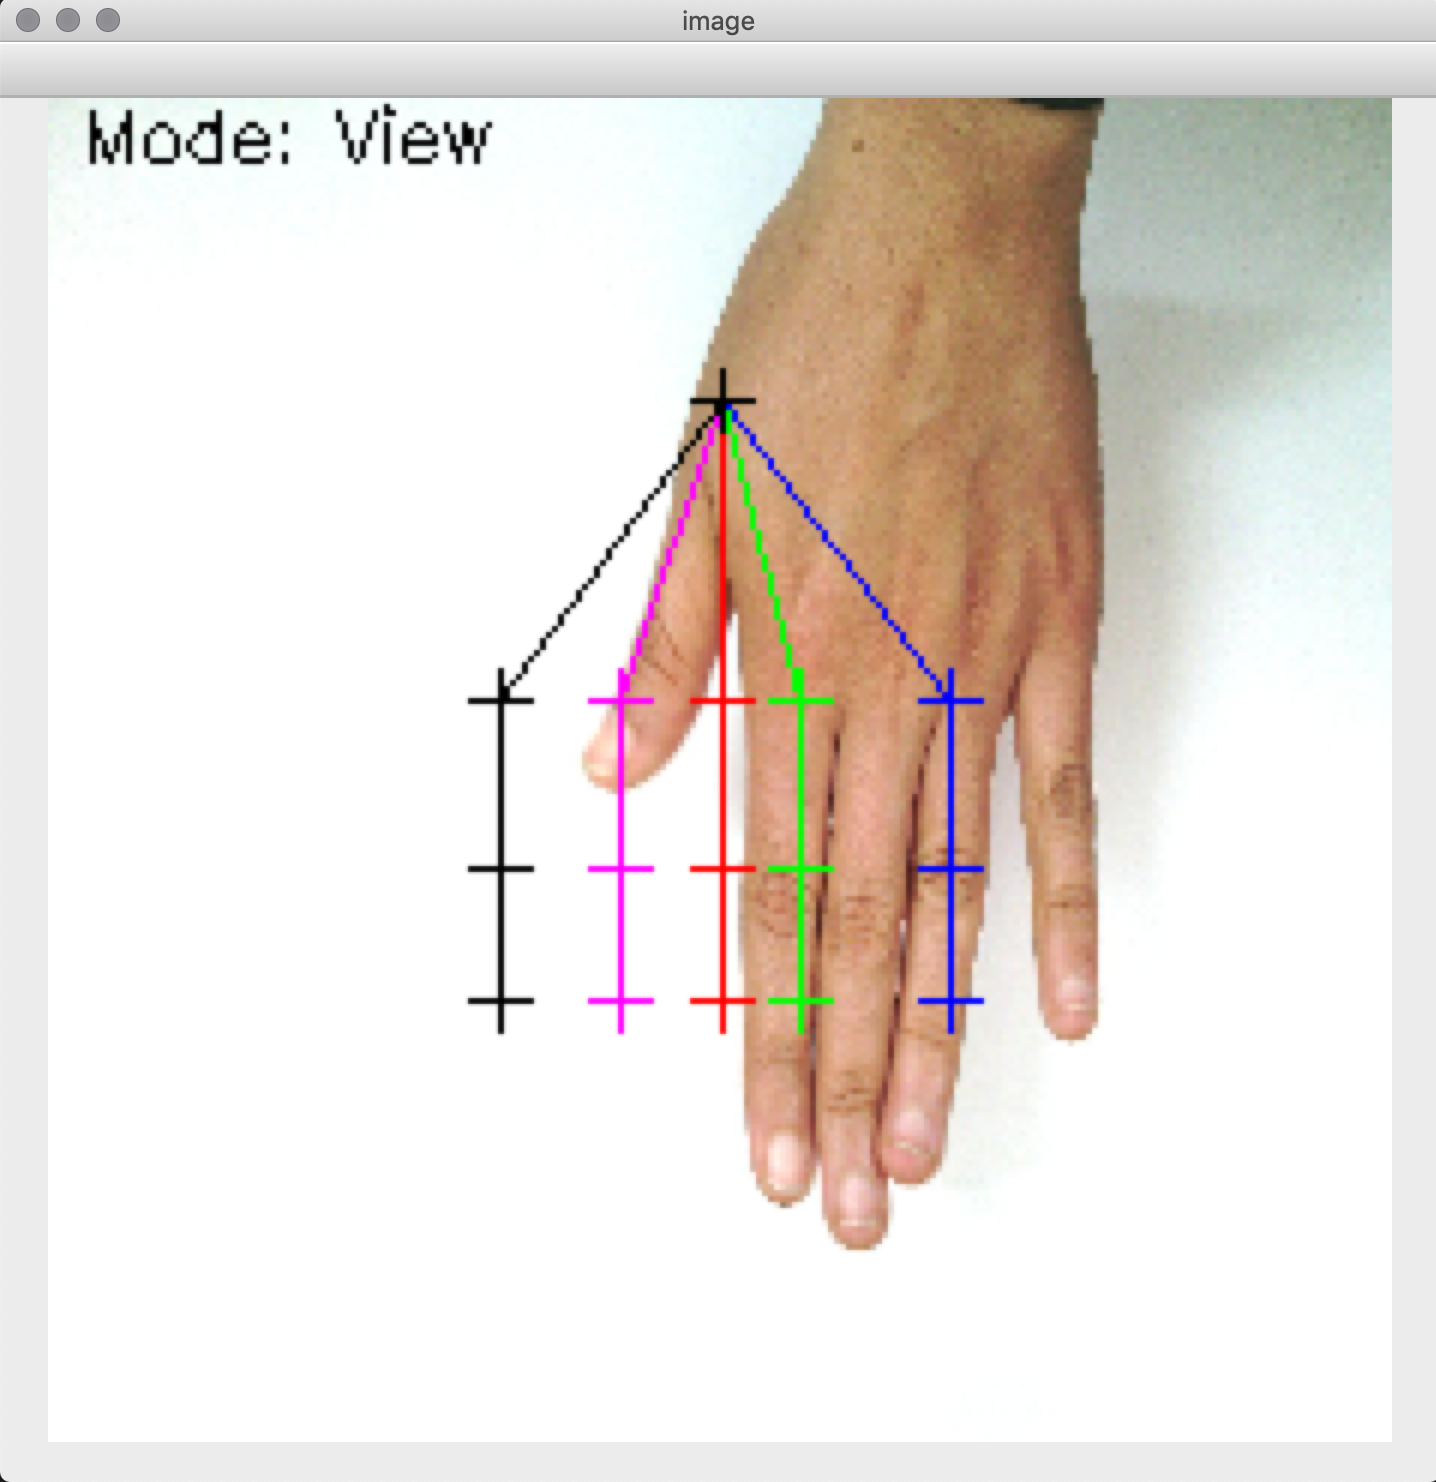
\includegraphics[width=0.25\linewidth]{./imgs/start.png}
  \end{center}
	\caption{スタート画面}
	\label{fig:startup}
\end{figure}

ツールはVIEW, SEQUENTIAL, EDIT, ROOTの4つのモードがありVIEWモードのときにnを押下すると次の画像を表示,sを押下すると座標を保存する.その他のモードで画像をクリックするとkey pointを設定できるようになっており,SEQUENTIALモードではすべての key point を連続して設定,EDITモードでは 0-4 に応じて親指から小指の付け根以外を設定,ROOTモードでは指の付け根を設定することができる.それぞれのモードは a, 0-4, r を押下すると切り替わり,該当するkey point を設定し終わるかESCを押下するとVIEWモードに戻る.各モードの選択時は\figref{fig:set_keypoints}のようになる.

\begin{figure}[H]
  \begin{center}
    \subfigure[SEQUENTIAL]{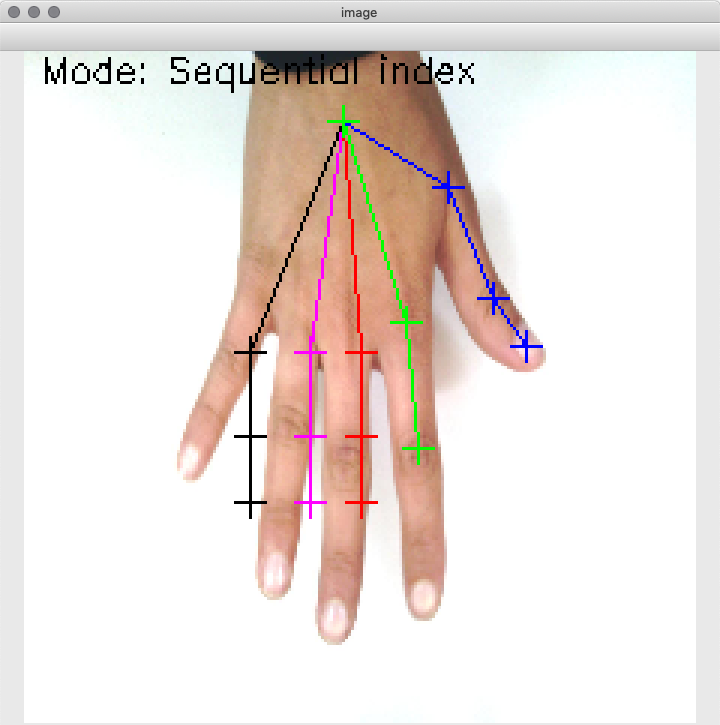
\includegraphics[width=0.25\linewidth]{./imgs/sequential.png}}
    \subfigure[EDIT]{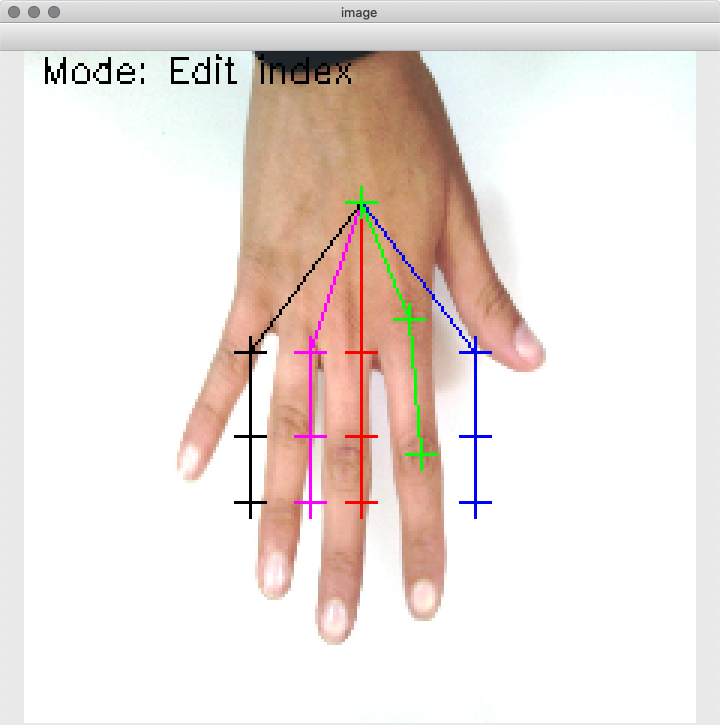
\includegraphics[width=0.25\linewidth]{./imgs/edit.png}}
    \subfigure[ROOT]{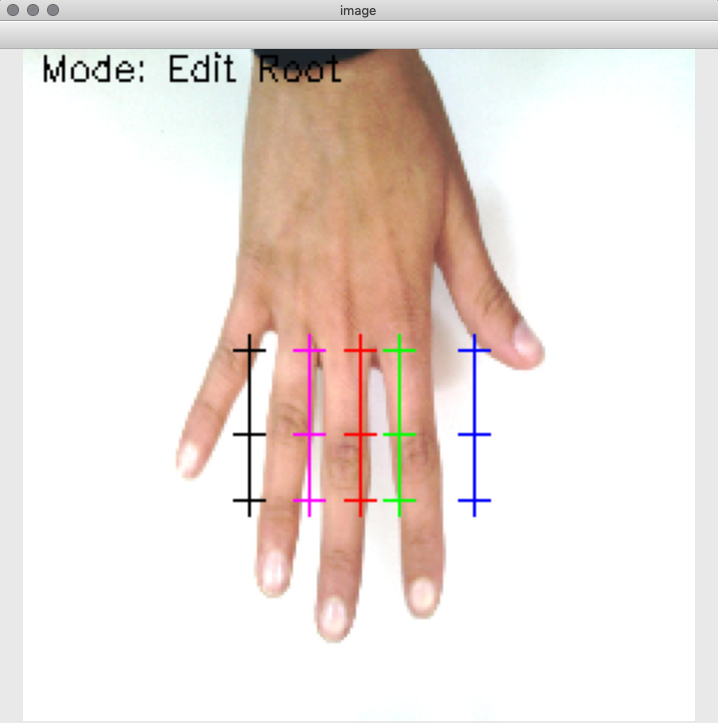
\includegraphics[width=0.25\linewidth]{./imgs/root.png}}
  \end{center}
	\caption{各モード選択時}
	\label{fig:set_keypoints}
\end{figure}

\subsection*{あると便利な機能}
アノテーション作業を中断,再開できるように簡単なログ機能を追加した.座標を保存した画像は次回起動時には読み込まれなくなるようになっており,アノテーションを再開するにはログファイルから該当するファイル名を削除すればよい.

\section*{課題2 CNNを用いて手のポーズを予測}
実行方法はREADME.mdの通りであり,

\begin{lstlisting}[language=bash]
  $ python predict.py -t [timestamp]
\end{lstlisting}

を実行後に

\begin{lstlisting}[language=bash]
  $ python annotate.py -p
\end{lstlisting}

を実行するとtrainデータの予測結果がデフォルトの座標としてアノテーションツールが起動する.実行結果を\figref{fig:predicted}に示す.

\begin{figure}[H]
  \begin{center}
    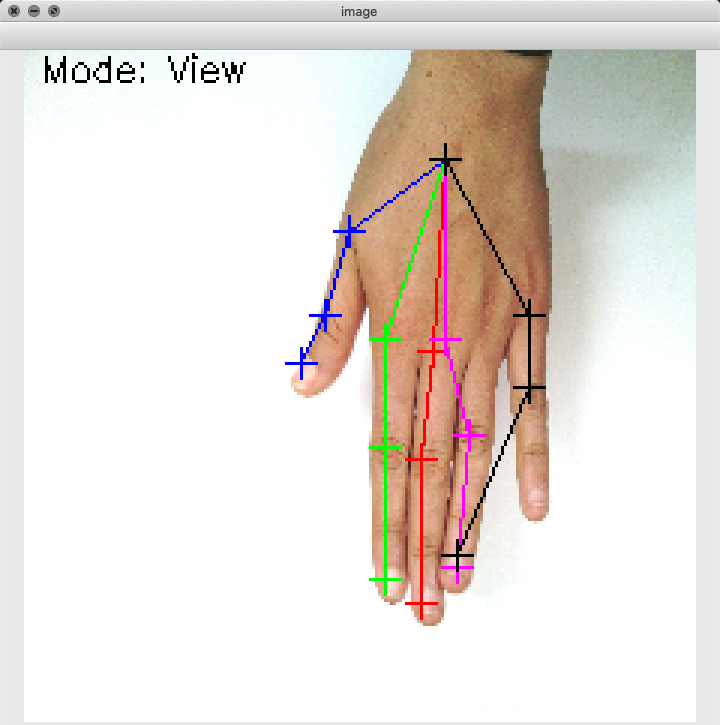
\includegraphics[width=0.25\linewidth]{./imgs/predicted.png}
  \end{center}
	\caption{予測結果の読み込み}
  \label{fig:predicted}
\end{figure}

\subsection*{課題で提示された手順に加えて適用して更に精度を上げるための手法}
\begin{itemize}
  \item key piintだけでなくそれぞれのkey pointが結ぶエッジも合わせて予測するネットワークを追加する\\
    予測されたエッジ端点や,エッジ同士の交点と対応するkey pointとの平均を予測結果とすることでよりノイズに頑健でロバストな学習結果を得られると考えられる.
\end{itemize}

\end{document}
